\chapter{Proof-of-Concept}%
\label{ch:poc}
Voor het eerste praktische deel van deze bachelorproef werden er drie virtuele machines opgezet binnen VirtualBox met behulp van Vagrant om een gecontroleerde testomgeving te creëren. Deze virtuele machines (VM’s) simuleren een scenario waarin een ransomware-aanval gericht wordt op databases die door het bedrijf worden beheerd. Het primaire doel van deze simulatie is aan te tonen dat het gebruik van immutable storage een effectieve maatregel kan zijn om belangrijke data te beschermen tegen ransomware-aanvallen.
\subsection{Relevantie van de PoC voor de Azure-omgeving van Forvis Mazars}
De Proof-of-Concept (PoC) in VirtualBox simuleert een ransomware-aanval in een lokale omgeving, gericht op het evalueren van beveiligingsmaatregelen zoals immutable storage. Deze aanpak sluit nauw aan bij de Azure-omgeving van Forvis Mazars, waar databases en back-ups worden beheerd.

De technieken uit de PoC, zoals immutable storage, kunnen direct worden toegepast in Azure via functies zoals immutable blobs in Azure Storage. Dit maakt het mogelijk om gegevens beter te beschermen tegen wijzigingen of verwijdering. Daarnaast biedt de PoC een veilig platform om de impact van een ransomware-aanval te begrijpen en te testen hoe snel en effectief back-ups kunnen worden hersteld, wat een cruciaal aspect is voor de bedrijfscontinuïteit.

Forvis Mazars kan de PoC gebruiken om risico’s te analyseren en beveiligingsoplossingen eerst kleinschalig te testen, alvorens deze op grotere schaal binnen hun cloudinfrastructuur toe te passen. Hiermee helpt de PoC bij het verfijnen en optimaliseren van hun bestaande Azure-back-upstrategie.
\subsection{Technische uitwerking}
Voor het opzetten van de virtuele machines in de Proof-of-Concept (PoC) werd gebruik gemaakt van een Vagrantfile. De Vagrantfile definieert de specificaties en configuraties van de VM’s, zoals geheugen, CPU, netwerkadapters en besturingssysteem. 
\begin{lstlisting}[language=Ruby, caption={Vagrantfile voor drie VM's: Back-up Server, Client, en Attacker}]
Vagrant.configure("2") do |config|

# Primary VM
config.vm.define "primary" do |primary|
primary.vm.box = "ubuntu/jammy64"

primary.vm.network "private_network", ip: "192.168.0.10", virtualbox__intnet: "internal_network"

primary.vm.provider "virtualbox" do |vb|
vb.memory = "2048" 
vb.cpus = 1        
end
end

# Back-up VM
config.vm.define "backup" do |backup|
backup.vm.box = "ubuntu/jammy64"

backup.vm.network "private_network", ip: "192.168.0.20", virtualbox__intnet: "internal_network"

backup.vm.provider "virtualbox" do |vb|
vb.memory = "2048" 
vb.cpus = 1       
end
end

# Attacker VM
config.vm.define "attacker" do |attacker|
attacker.vm.box = "ubuntu/jammy64"

attacker.vm.network "private_network", ip: "192.168.0.30", virtualbox__intnet: "internal_network"

attacker.vm.provider "virtualbox" do |vb|
vb.memory = "1024" 
vb.cpus = 1        
end
end

end
\end{lstlisting}

In de onderstaande tabel worden de specificaties van de drie virtuele machines weergegeven die in de Proof-of-Concept zijn gebruikt. Elke VM heeft een specifieke functie binnen het netwerk. De tabel bevat details over de hoeveelheid toegewezen RAM, het aantal CPU-cores, het gebruikte besturingssysteem, de toegewezen IP-adressen en de configuratie van de netwerkadapter. Deze configuratie zorgt ervoor dat de VM's binnen hetzelfde interne netwerk met elkaar kunnen communiceren, wat essentieel is voor het testen van de ransomware-aanval en de back-upstrategieën.
\begin{longtable}{|l|c|c|c|l|l|}
    \hline
    \textbf{Functie} & \textbf{RAM} & \textbf{CPU Cores} & \textbf{IP} & \textbf{Besturingssysteem} & \textbf{Netwerkadapter} \\ \hline
    Primary server    & 2 GB         & 1                  & 192.168.0.10 & Ubuntu 22.04.5 LTS & NAT + Internal \\ \hline
    Back-up server           & 1 GB         & 1                  & 192.168.0.20 & Ubuntu 22.04.5 LTS & NAT + Internal \\ \hline
    Attacker VM         & 2 GB         & 1                  & 192.168.0.30 & Ubuntu 22.04.5 LTS     & NAT + Internal \\ \hline
    
\caption{Beschrijving van de virtuele machines in de Proof of Concept}
\end{longtable}

De Primary VM stelt een actieve databankserver voor binnen een bedrijfsomgeving. Deze server bevat de operationele data van het bedrijf en vertegenwoordigt de belangrijkste bron die beschermd moet worden tegen dataverlies of aanvallen. 

De Back-up VM fungeert als een back-upserver waarop regelmatig de databankback-ups worden opgeslagen. Deze back-upserver is cruciaal voor bedrijfscontinuïteit en disaster recovery, omdat ze in geval van een aanval of fout de herstelmogelijkheden biedt. 

De Attacker VM vertegenwoordigt een hacker met slechte intenties binnen de testomgeving. Deze machine wordt gebruikt om een ransomware-aanval te simuleren, waarbij de functionaliteit van zowel de Primary VM als de Back-up VM wordt bedreigd. Het doel van deze opstelling is om te demonstreren hoe een back-upstrategie, inclusief technieken zoals immutable storage, een bedrijf kan beschermen tegen de gevolgen van een dergelijke aanval.
\subsubsection{Aanmaken van de database}
Op de primary VM werd een eenvoudige SQL-database geïnstalleerd en de volgende tabel aangemaakt om als testdata te dienen:
\begin{lstlisting}[language=SQL, caption={MySQL-code voor het aanmaken van de testdatabank}]
CREATE TABLE employees (
    id INT AUTO_INCREMENT PRIMARY KEY,
    name VARCHAR(50),
    role VARCHAR(50)
);
INSERT INTO employees (name, role) VALUES 
    ('Alice', 'Engineer'), 
    ('Bob', 'Manager'), 
    ('Charlie', 'Analyst');
\end{lstlisting}



\subsubsection{Back-up van de database}
Nadien werd de database geëxporteerd naar een \texttt{.sql}-bestand met het volgende \texttt{mysqldump}-commando:
\begin{lstlisting}[language=script, caption={mysqldump commando om een databank te exporteren}]
mysqldump -u testuser -p testdb > /home/vagrant/backup.sql
\end{lstlisting}
Het resulterende bestand, \texttt{backup.sql}, werd vervolgens met BorgBackup opgeslagen in een back-uprepository op de back-up VM. De repository werd vooraf geïnitialiseerd met het volgende commando:
\begin{lstlisting}[language=script, caption={Borg commando om een map te initialiseren als Borg repository}]
borg init --encryption=repokey /home/vagrant/backups
\end{lstlisting}
Vervolgens werd de back-up gemaakt:
\begin{lstlisting}[language=script, caption={Borg commando om een back-up te nemen}]
borg create --progress 
ssh://vagrant@192.168.0.20/home/vagrant/backups::backup-$(date +%Y-%m-%d) 
/home/vagrant/backup.sql
\end{lstlisting}

\subsubsection{Beveiliging van de back-updirectory}
Om de back-updirectory ransomware-resistent te maken, werd het Linux-commando \texttt{chattr} gebruikt om het \textit{immutable}-attribuut toe te passen op de back-updirectory. Dit attribuut zorgt ervoor dat er geen wijzigingen aan de bestanden in de directory gebeuren, zelfs door gebruikers met \texttt{root}-rechten. Het commando:
\begin{lstlisting}[language=script, caption={Linux commando om de map immutable te maken}]
sudo chattr +i /home/vagrant/backups/
\end{lstlisting}

\subsubsection{Simulatie van de ransomware-aanval}
Op de attacker VM werd een script gebruikt om de ransomware-aanval te simuleren. Het script probeert alle bestanden in de back-updirectory te hernoemen door \texttt{.malware} toe te voegen aan de bestandsnamen. Dit zou overeenkomen met een ransomware-aanval waarbij de back-up bestanden geëncrypteerd worden. Het script is hieronder weergegeven:
\begin{lstlisting}[language=script, caption={Bash script om een ransomware-aanval na te bootsen}]
#!/bin/bash
    
BACKUP_DIR="/home/vagrant/backups"
    
for file in "$BACKUP_DIR"/*; do
  if [ -f "$file" ]; then
    if mv "$file" "${file}.malware"; then
      echo "Renamed $file to ${file}.malware"
    else      
      echo "Error: Could not rename $file"    
    fi    
  fi    
done    
\end{lstlisting}
Voor het gemak heeft de Attacker VM volledige controle gekregen over de Back-up VM. Dit is gedaan omdat de scope van deze bachelorproef niet is om toegang te verkrijgen tot een server, maar eerder om een gecontroleerde omgeving te creëren waarin een Attacker VM een ransomware-aanval nabootst. Het doel is te demonstreren hoe de ransomware zich verspreidt naar de back-up directory, en niet om de daadwerkelijke methoden voor het verkrijgen van toegang tot een server in detail uit te werken.

Toen dit script werd uitgevoerd op de back-up VM, werd duidelijk dat het hernoemen van de bestanden niet lukte vanwege het immutable-attribuut. Dit toont aan dat de ransomware-aanval niet slaagde en de bestanden in de back-updirectory beschermd bleven.

\subsubsection{Herstellen van de back-ups}
Om te bewijzen dat de back-ups nog steeds bruikbaar waren, werd een herstelproces uitgevoerd op de primary VM vanuit de Borg-repository:
\begin{lstlisting}[language=script, caption={Borg commando om een back-up te herstellen}]
borg extract 
ssh://vagrant@192.168.0.20/home/vagrant/backups::backup-2024-12-05
\end{lstlisting}

De databank werd opnieuw opgezet vanuit het bestand dat uit de Borg-repository werd gehaald met het volgende commando:
\begin{lstlisting}[language=script, caption={MySQL commando om een databank te herstellen vanuit een .sql-bestand}]
mysql -u root -p restored_db < /home/vagrant/backup.sql
\end{lstlisting}
De back-up werd gebruikt om de database te herstellen en te controleren. Het herstelproces verliep succesvol, wat bewijst dat de immutable storage de integriteit van de back-ups had behouden en dat de bestanden veilig waren gebleven ondanks de ransomware-aanval.

\newpage
\subsection{Implementatie van immutable storage in de Azure-omgeving}
\subsubsection{Aanmaken van een storage account}
De eerste stap in het implementeren van Immutable Storage in Azure is het aanmaken van een \texttt{Storage Account} in de Azure Portal. 
\begin{figure}[h]
    \centering
    \captionsetup{justification=centering}    
    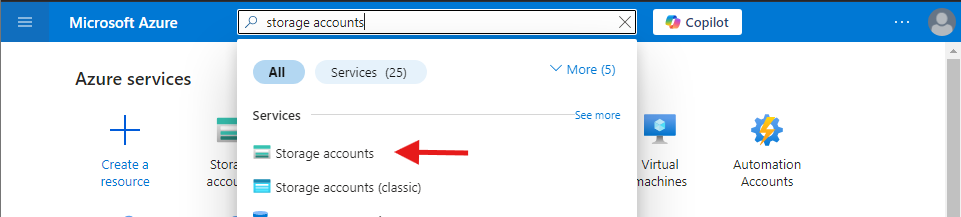
\includegraphics[width=0.8\textwidth]{img/1imm.png}
    \caption{Storage account zoekopdracht binnen de Azure Portal}
\end{figure}
Bij het aanmaken van het storage account kiezen we de correcte resource group, naam die het account moet krijgen, regio en bij redundancy kiezen we voor \texttt{Locally-redundant storage (LRS)}. Bij de optie \texttt{Account kind} kiezen we voor \texttt{General-purpose v2}, omdat deze versie alle benodigde functionaliteit biedt, zoals het ondersteunen van de blob storage en het configureren van immutability policies. 
\begin{figure}[h]
    \centering
    \captionsetup{justification=centering}    
    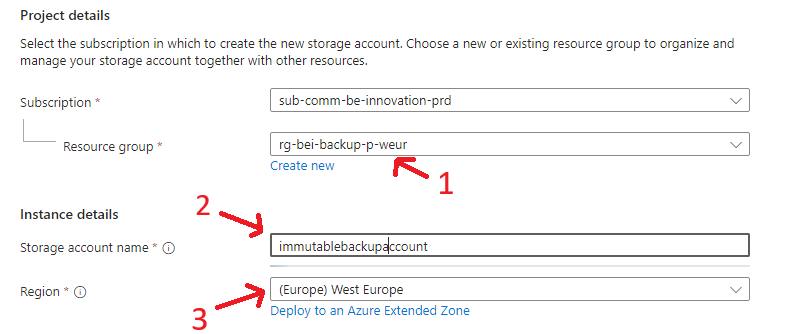
\includegraphics[width=0.8\textwidth]{img/3.1imm.png}
    \caption{Configuratie voor het nieuwe storage account}
\end{figure}
\begin{figure}[h]
    \centering
    \captionsetup{justification=centering}    
    
\includegraphics[width=0.8\textwidth]{img/3.2imm.png}
    \caption{Tweede deel van de configuratie voor het nieuwe storage account}
\end{figure}
\newpage
\subsubsection{Aanmaken van een container binnen het storage account}
Na het aanmaken van het storage account moet er een container geconfigureerd worden binnen het nieuwe storage account om de gegevens op te slaan. Bij het aanmaken van de container moet de \texttt{public access level} op private staan voor de veiligheid. Containers in Azure werken als mappen waarin je blobs kunt opslaan zoals back-ups.
\begin{figure}[h]
    \centering
    \captionsetup{justification=centering}    
    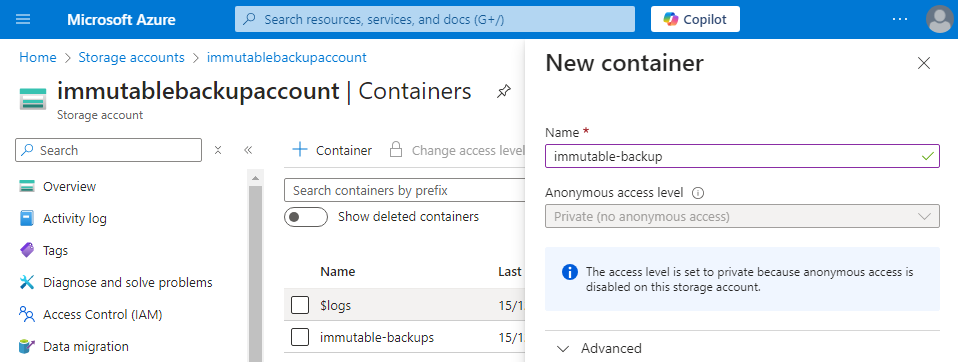
\includegraphics[width=0.8\textwidth]{img/4imm.png}
    \caption{Configuratie voor de container in het storage account}
\end{figure}
\subsubsection{Opzetten van een time-based retention policy}
Nadien moet er een immutability policy opgezet worden. Hierbij werd gekozen voor een time-based retention policy van 90 dagen, de back-up is met andere woorden bescherm tegen verwijdering of wijziging voor deze periode. Dit is een veilige en praktische keuze voor back-ups. Daarnaast is er bij de optie \texttt{ Allow protected append writes to } gekozen voor \texttt{ Block and append blobs}, dit maakt het mogelijk om gegevens te blijven toevoegen aan de blob zonder de bestaande gegevens te wijzigen of te verwijderen, wat ideaal is voor scenario's zoals logbestanden of incrementele back-ups.
\begin{figure}[h]
    \centering
    \captionsetup{justification=centering}    
    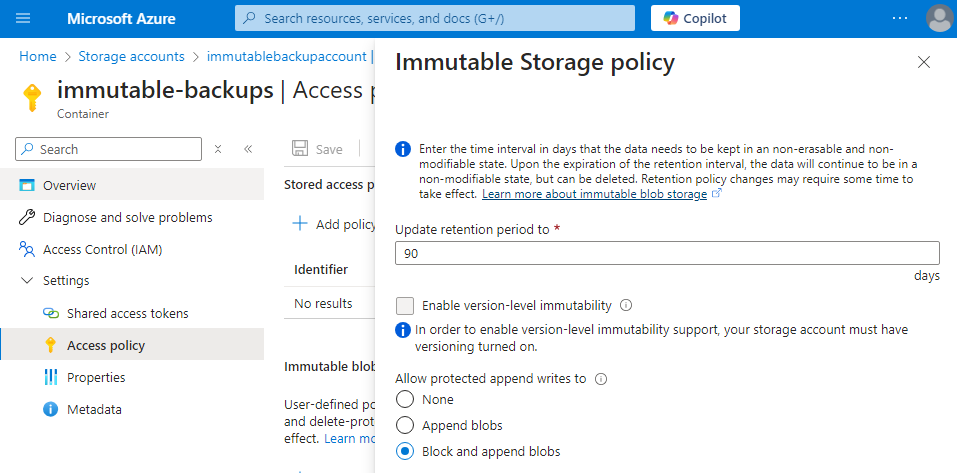
\includegraphics[width=0.8\textwidth]{img/6imm.png}
    \caption{Configuratie voor time-based retention policy}
\end{figure}
\newpage
\subsubsection{Testen van de immmutable storage}
Om de immutable storage te testen is er gekozen om een back-up van een MySQL-database de uploaden naar de container. Na het uploaden van het bestand was er geen optie om dit bestand te verwijderen of te wijzigen. Met andere woorden is deze back-up dus beschermd tegen een ransomware-aanval.
\begin{figure}[h]
    \centering
    \captionsetup{justification=centering}    
    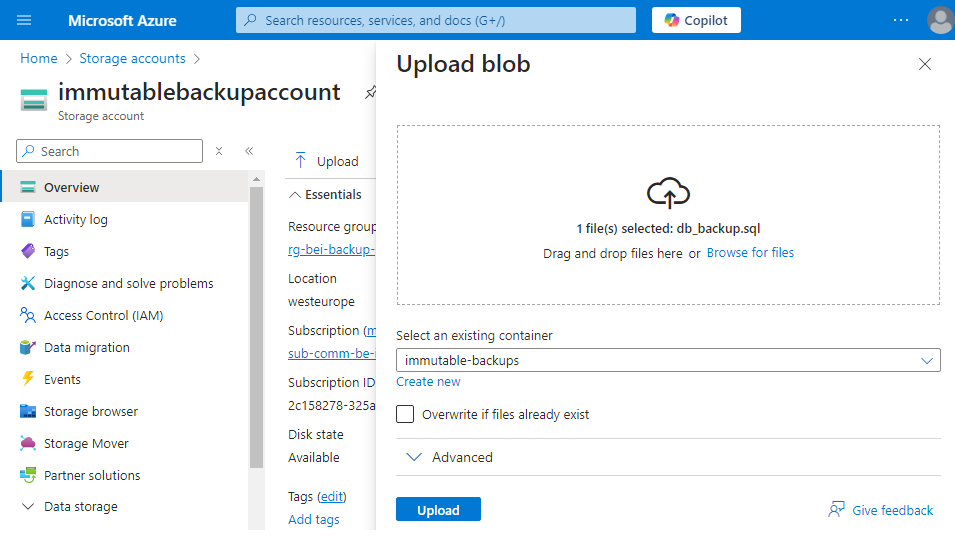
\includegraphics[width=0.8\textwidth]{img/7imm.png}
    \caption{Uploaden van het back-up bestand van de MySQL-databank}
\end{figure}
\begin{figure}[h]
    \centering
    \captionsetup{justification=centering}    
    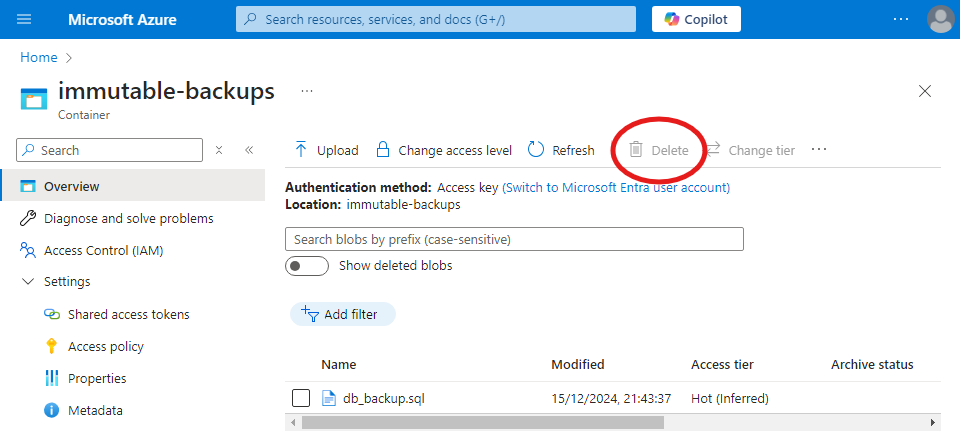
\includegraphics[width=0.8\textwidth]{img/8imm.png}
    \caption{Screenshot van de poging om het bestand te verwijderen, waarbij de actie wordt geblokkeerd}
\end{figure}
\subsubsection{Conclusie}
De implementatie van immutable storage op het azure storage account is succesvol afgerond, waardoor de opgeslagen back-ups nu beschermd zijn tegen onverwachte wijzigingen of verwijderingen. Daarnaast worden er dagelijks automatische back-ups van de databanken genomen, welke een retentieperiode van 7 dagen hebben. Dit zorgt ervoor dat er altijd een versie van de back-up beschikbaar is, zelfs als de meest recente back-up beschadigd of onbruikbaar blijkt. Deze combinatie van immutable storage en versiebeheer versterkt de bescherming tegen dataverlies en maakt het mogelijk om eerdere, werkende back-ups snel te herstellen.


\subsection{Implementatie van de Kubernetes-gebaseerde automatische back-upoplossing}

\subsubsection{Inleiding}
In mijn Proof of Concept (PoC) maak ik gebruik van een Kubernetes-omgeving om een schaalbare, geautomatiseerde back-upoplossing te realiseren voor PostgreSQL- en MySQL-databases. Deze databases draaien lokaal op een Vagrant Virtual Machine (VM), wat het testproces vereenvoudigt en isolatie biedt voor de back-upworkflow. De back-ups worden uitgevoerd door containers die draaien binnen Kubernetes Pods. De containers maken gebruik van een op maat gemaakte Docker-image die een Python-script bevat voor het uitvoeren van de back-ups en het opschonen van oude bestanden.

Kubernetes speelt een centrale rol in deze oplossing door de automatisering van de back-upworkflow via \textbf{CronJobs}, het beheer van opslag via \textbf{Persistent Volumes (PV)} en \textbf{Persistent Volume Claims (PVC)}, en de beveiliging van gevoelige gegevens via \textbf{Secrets}. Deze componenten werken samen om een robuuste en herhaalbare oplossing te bieden.

In deze tekst worden de configuraties, werking van de Kubernetes Pods en de samenwerking tussen de Docker-image en Kubernetes toegelicht.

\subsubsection{Kubernetes Pods en Werking}
Een \textbf{Kubernetes Pod} is de kleinste uitvoereenheid binnen een Kubernetes-cluster. Elke Pod bevat een of meer containers die een specifieke taak uitvoeren. In dit project wordt een Pod geconfigureerd om:
\begin{itemize}
    \item De back-up van een database uit te voeren.
    \item Data op te slaan in een Persistent Volume.
    \item Gevoelige informatie, zoals wachtwoorden, te beheren via Secrets.
\end{itemize}

Voor elke database (PostgreSQL en MySQL) is een aparte CronJob geconfigureerd. Deze CronJobs maken gebruik van dezelfde Docker-image, maar passen specifieke parameters toe om de juiste database te back-uppen.

Het proces verloopt als volgt:
\begin{enumerate}
    \item De CronJob wordt volgens een gepland schema uitgevoerd.
    \item De CronJob spint een Pod op waarin de container draait die de back-up uitvoert.
    \item De container voert het Python-script uit dat de database-back-up naar een Persistent Volume schrijft.
    \item Na voltooiing wordt de Pod beëindigd, terwijl de back-upbestanden bewaard blijven.
\end{enumerate}

\subsubsection{Persistent Volume en Persistent Volume Claim}

De back-ups worden opgeslagen op een Persistent Volume dat is gekoppeld aan een directory op de hostmachine van de Vagrant VM. Hierdoor blijven de gegevens bewaard, zelfs als de Kubernetes Pods opnieuw worden gestart.

\subsubsection*{Persistent Volume}
\begin{lstlisting}[language=yaml, caption=Persistent Volume Configuratie]
    apiVersion: v1
    kind: PersistentVolume
    metadata:
    name: backup-pv
    spec:
    capacity:
    storage: 5Gi
    accessModes:
    - ReadWriteOnce
    persistentVolumeReclaimPolicy: Retain
    storageClassName: ""
    hostPath:
    path: "/data"  # Windows path
\end{lstlisting}

\textbf{Toelichting:}
\begin{itemize}
    \item \texttt{hostPath}: De directory \texttt{/data} op de hostmachine (Vagrant VM) wordt gebruikt voor opslag.
    \item \texttt{persistentVolumeReclaimPolicy}: Met \texttt{Retain} blijven gegevens behouden, zelfs als de PVC wordt verwijderd.
\end{itemize}

\subsubsection*{Persistent Volume Claim}
\begin{lstlisting}[language=yaml, caption=Persistent Volume Claim Configuratie]
    apiVersion: v1
    kind: PersistentVolumeClaim
    metadata:
    name: backup-pvc
    spec:
    accessModes:
    - ReadWriteOnce
    resources:
    requests:
    storage: 5Gi
    storageClassName: ""
\end{lstlisting}

\textbf{Toelichting:}
\begin{itemize}
    \item De PVC koppelt het Persistent Volume aan de Pod, zodat de back-ups toegankelijk zijn vanuit de container.
\end{itemize}

\subsubsection{Dockerfile en Samenwerking met Kubernetes}

De Docker-image die door de Kubernetes Pods wordt gebruikt, is gebaseerd op een aangepaste Dockerfile. Deze bevat alle benodigde tools en het Python-script dat de back-ups uitvoert. Hier is de configuratie van de Dockerfile:

\begin{lstlisting}[language=docker, caption=Dockerfile Configuratie]
    FROM ubuntu:20.04
    
    RUN apt-get update && apt-get install -y \
    mysql-client \
    postgresql-client \
    python3 \
    python3-pip \
    && rm -rf /var/lib/apt/lists/*
    
    COPY backup_script.py /backup_script.py
    RUN chmod +x /backup_script.py
    
    WORKDIR /
    
    ENTRYPOINT ["python3", "/backup_script.py"]
\end{lstlisting}

\textbf{Toelichting:}
\begin{itemize}
    \item \textbf{Base image}: De image is gebaseerd op \texttt{ubuntu:20.04}.
    \item \textbf{Installatie van tools}: De benodigde database-clients (MySQL en PostgreSQL) en Python worden geïnstalleerd.
    \item \textbf{Kopie van script}: Het back-upscript (\texttt{backup\_script.py}) wordt in de image opgenomen en uitvoerbaar gemaakt.
    \item \textbf{ENTRYPOINT}: Dit stelt de standaardopdracht in die wordt uitgevoerd bij het starten van de container.
\end{itemize}

\textbf{Samenwerking met Kubernetes Pods:}
\begin{itemize}
    \item \textbf{CronJob}: Bij het starten van een Pod door een CronJob, wordt de Docker-image uitgevoerd.
    \item \textbf{Command Parameters}: Kubernetes CronJobs kunnen specifieke parameters aan de container doorgeven (bijvoorbeeld de databasenaam, gebruiker, en type).
    \item \textbf{Persistent Volume}: De container heeft toegang tot het Persistent Volume via een volume-mount, zodat de back-ups persistent worden opgeslagen.
\end{itemize}

\subsubsection{PostgreSQL Back-up CronJob}

De PostgreSQL-back-up wordt uitgevoerd met de eerder genoemde Docker-image en het Python-script. De CronJob is geconfigureerd om dagelijks om 2:00 uur een back-up uit te voeren.

\begin{lstlisting}[language=yaml, caption=CronJob voor PostgreSQL-back-up]
    apiVersion: batch/v1
    kind: CronJob
    metadata:
    name: backup-psql-cronjob
    spec:
    schedule: "0 2 * * *"  
    jobTemplate:
    spec:
    ttlSecondsAfterFinished: 3600  
    template:
    spec:
    containers:
    - name: backup-psql-container
    image: bouzewazi/ubu4
    command: 
    - "python3"
    - "/backup_script.py"
    - "-dn"
    - "testdb"
    - "-du"
    - "root"
    - "-t"
    - "PSQL"
    - "-b"
    - "-bd"
    - "/data"
    volumeMounts:
    - name: backup-storage
    mountPath: /data  
    env:
    - name: PGPASSWORD
    valueFrom:
    secretKeyRef:
    name: db-secret2
    key: PGPASSWORD
    resources:
    requests:
    memory: "1Gi"  
    cpu: "250m"      
    limits:
    memory: "2Gi"  
    cpu: "500m"      
    restartPolicy: OnFailure
    volumes:
    - name: backup-storage
    persistentVolumeClaim:
    claimName: backup-pvc
\end{lstlisting}

\subsubsection{Opschonings-CronJob}

Om oude back-ups te verwijderen, wordt een opschonings-CronJob gebruikt die het Python-script aanroept met de \texttt{-r}-optie.

\begin{lstlisting}[language=yaml, caption=Opschonings-CronJob Configuratie]
    apiVersion: batch/v1
    kind: CronJob
    metadata:
    name: delete-cronjob
    spec:
    schedule: "0 2 * * *"  
    jobTemplate:
    spec:
    ttlSecondsAfterFinished: 3600  
    template:
    spec:
    containers:
    - name: delete-backup-container
    image: bouzewazi/ubu4
    command: 
    - "python3"
    - "/backup_script.py"
    - "-dn"
    - "testdb"
    - "-du"
    - "root"
    - "-t"
    - "MYSQL"
    - "-r"
    - "14"  # Retentieperiode van 14 dagen
    - "-bd"
    - "/data"
    volumeMounts:
    - name: backup-storage
    mountPath: /data  
    env:
    - name: DB_PASSWORD
    valueFrom:
    secretKeyRef:
    name: db-secret
    key: DB_PASSWORD
\end{lstlisting}

\textbf{Toelichting:}
\begin{itemize}
    \item \textbf{Retentieperiode}: Back-ups ouder dan 14 dagen worden verwijderd.
    \item \textbf{CronJob-samenwerking}: De opschonings-CronJob werkt samen met het Persistent Volume en gebruikt dezelfde directory (\texttt{/data}) als de back-ups.
    \end


\subsubsection{Relevantie voor Forvis Mazars}
Deze oplossing kan eenvoudig worden geïntegreerd in de infrastructuur van Forvis Mazars, omdat het gebruik maakt van Docker-containers. Forvis Mazars beheert hun back-ups binnen een Kubernetes-cluster, en Docker-containers kunnen rechtstreeks als pods worden gedeployed in Kubernetes. Hierdoor kan de huidige oplossing zonder aanpassingen worden hergebruikt. De setup in deze implementatie, waarbij de databases op een virtuele machine draaien en de back-ups worden uitgevoerd via Docker-containers, komt overeen met de werkomgeving van Forvis Mazars. Dit zorgt ervoor dat de voorgestelde oplossing naadloos aansluit op hun huidige infrastructuur en gebruiksbehoeften.


\subsection{Herstelcapaciteit (Restore from Backup)}
Een belangrijk onderdeel van het praktijkgedeelte van dit onderzoek is het testen van de \textbf{herstelcapaciteit} (Restore from Backup). Dit was een essentiële vereiste in het onderzoek, waarbij de focus lag op het efficiënt en snel herstellen van systemen vanuit de back-ups. Het doel was om een idee te krijgen over hoe snel en betrouwbaar een databank up-and-running kan zijn na het ondergaan van een incident.

\subsubsection{Toepassing van de Herstelstrategie}
Om deze must-have te evalueren, heb ik de gehele herstelprocedure in een gecontroleerde testomgeving uitgevoerd. Deze testomgeving komt grotendeels overeen met de actieve omgeving die Forvis Mazars gebruikt. Dit proces omvatte de volgende stappen:

\begin{enumerate}
    \item \textbf{Back-ups ophalen uit de immutable storage in Azure} \\
    De back-ups werden veilig opgeslagen in een Azure Storage Account met een immutable opslagbeleid, wat een cruciale maatregel is tegen ransomware-aanvallen. Door het gebruik van het \texttt{az storage blob download}-commando werden de back-ups gedownload naar de lokale virtuele machine.
    
    \item \textbf{Herstellen van de PostgreSQL- en MySQL-databanken} \\
    Na het downloaden werden de PostgreSQL- en MySQL-databases opnieuw opgezet met herstelcommando’s. Voor PostgreSQL werd het bestand hersteld met \texttt{pg\_restore}, terwijl voor MySQL gebruik werd gemaakt van het \texttt{mysql}-commando. Beide hersteltaken verliepen succesvol en zonder dataverlies, waarmee de betrouwbaarheid van de back-upstrategie werd aangetoond. Dit hele proces is gemeten en duurde ongeveer \textbf{23 seconden}, wat wijst op een snelle toegang tot de back-ups in noodsituaties.
\end{enumerate}

\subsubsection{Link met Herstelcapaciteit}
De testprocedure toont aan dat de opgestelde back-upstrategie niet alleen effectief is in het beschermen van gegevens, maar ook voldoet aan de eisen van herstelcapaciteit:

\begin{itemize}
    \item \textbf{Efficiëntie:} Het herstelproces, vanaf het downloaden van de back-ups tot het opnieuw opzetten van de databases, verliep in een relatief korte tijd. Dit bevestigt dat de back-ups eenvoudig en snel toegankelijk zijn, wat essentieel is in een bedrijfsomgeving waar down-time zo laag mogelijk moet zijn.
    
    \item \textbf{Betrouwbaarheid:} Door gebruik te maken van immutable opslag in Azure worden de back-ups beschermd tegen ongewenste acties en aanvallen, wat de kans op succesvol herstel sterk verhoogt.
\end{itemize}

\subsubsection{Conclusie}
De uitgevoerde tests bieden waardevolle inzichten in de herstelcapaciteit van de back-upstrategie. Het toont aan hoe een goed ontworpen back-upplan bedrijven in staat stelt om snel te reageren op noodsituaties en hun systemen betrouwbaar te herstellen. Hiermee is aangetoond dat het systeem niet alleen beschermt tegen gegevensverlies, maar ook operationeel herstel mogelijk maakt binnen een acceptabele tijd. Dit maakt het een reële oplossing voor bedrijven die ransomware-resistente back-upstrategieën willen implementeren.































